\section{Distribución Binomial}

Supongamos que efectuamos una serie de $n$ ensayos independientes Bernoulli en
donde la probabilidad de éxito en cada ensayo es $p$. Si denotamos por $E$ el
resultado éxito y por $F$ el resultado fracaso, entonces el espacio muestral de
este experimento consiste de todas las posibles sucesiones de longitud $n$ de
caracteres $E$ y $F$ . Así, el espacio muestral consiste de $2^n$ elementos. Si
ahora definimos la variable aleatoria X como aquella función que indica el
número de éxitos en cada una de estas sucesiones, esto es,

\begin{equation}
    \begin{array}{ll}
        X(EE...EE) & = n, \\
        X(FE...EE) & = n-1, \\
        . & \\
        . & \\
        . & \\
        X(FF...FF) & = 0
    \end{array}
\end{equation}

entonces tenemos que $X$ puede tomar los valores 0, 1, 2, . . . , $n$, con las
probabilidades dadas por la función de probabilidad.

\begin{tcolorbox}[colback=gray!5!white,colframe=gray!60!black,title=Definición: Función de Distribución Binomial]
    La función de probabilidad de una distribución binomial se define como la
    probabilidad de que ocurran exactamente $x$ eventos exitosos de $n$ experimentos
    independientes de probabilidad $p$.

    \begin{equation}
      P(k) = \binom{n}{x} p^x q^{n-x}
    \end{equation}
    
    Esto a también es escrito como:
    \begin{equation}
      b(x; n,p) = \binom{n}{x} p^x q^{n-x}
    \end{equation}
    Donde $0 \leq x \leq n$

    Probabilidad de "éxito": $p$

    Probabilidad de "fracaso": $q = 1 - p$
\end{tcolorbox}

Decimos entonces que $X$ tiene una distribución binomial con parámetros $n$ y
$p$, y escribimos $X \sim \text{bin}(n,p)$. Esta expresión para la función de
probabilidad puede obtenerse de la siguiente forma: la probabilidad de obtener
$x$ éxitos y $n-x$ fracasos en $n$ ensayos Bernoulli es,

\begin{equation}
    \underbrace{p...p}_{x} \underbrace{(1-p)...(1-p)}_{n-x} = p^x(1-p)^{n-x}.
\end{equation}

\subsection{Ejemplo de distribución Binomial}

Un jugador de baloncesto tiene un 80\% de acierto en tiros libres. Si tira tres
lanzamientos seguidos, ¿Cuál es la probabilidad de que acierte dos de los tres
lanzamientos?

Sabiendo que:\\

$p = 0.8$ y  $q = 0.2$

Entonces: \\

$P(\text{dos aciertos}) = P(A \cap A \cap \bar{A}) 
                      \cup P(A \cap \bar{A} \cap A)
                      \cup P(\bar{A} \cap A \cap A )$

Por lo que: \\
$P(A \cap A \cap \bar{A}) = p \cdot p \cdot q 
                          = 0.8 \cdot 0.8 \cdot 0.2 
                          = 0.128$

Así: \\

$P(\text{dos aciertos}) = 0.128 + 0.128 + 0.128 = 3 \cdot 0.128$

Notemos que:

$P(\text{dos aciertos}) = P(A \cap A \cap \bar{A}) 
                      \cup P(A \cap \bar{A} \cap A)
                      \cup P(\bar{A} \cap A \cap A )$
                      
Estamos haciendo una combinatoria:

$C(3,2)$

De esta manera podemos hacerlo para experimentos más grandes. Digamos, ¿cuál
sería la probabilidad de acertar 3 canastas si hiciera 15 lanzamientos?

$C(15,3) = 455$

Un jugador de baloncesto tiene un 80\% de acierto en tiros libres. Si tira 20
lanzamientos seguidos, ¿cuál es la probabilidad de que acierte 13 de los
lanzamientos?
  
$P(13) = C(20,13) 0.8^{13} \cdot 0.2^{7} = 0.0545$

Ahora podemos obtener la distribución de la probabilidad pasando por todos los
valores posibles desde 0 hasta $x$.

\begin{figure}[h!]
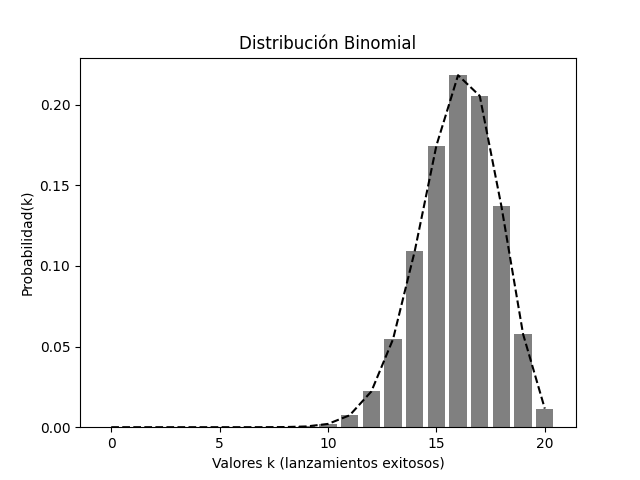
\includegraphics[scale=0.9]{../slides/figures/binomial_distribution.png}
\label{fig:binomial_distribution}
\caption{Gráfica de la función de probabilidad binomial con los parámetros $n=20$ y $p=0.8$}
\end{figure}

Cuando el éxito y el fracaso son igualmente probables, la distribución binomial
es una distribución normal. Por lo que si cambiamos el valor de $p$ a 0.5,
obtenemos la siguiente gráfica de distribución normal.

\begin{figure}[h!]
    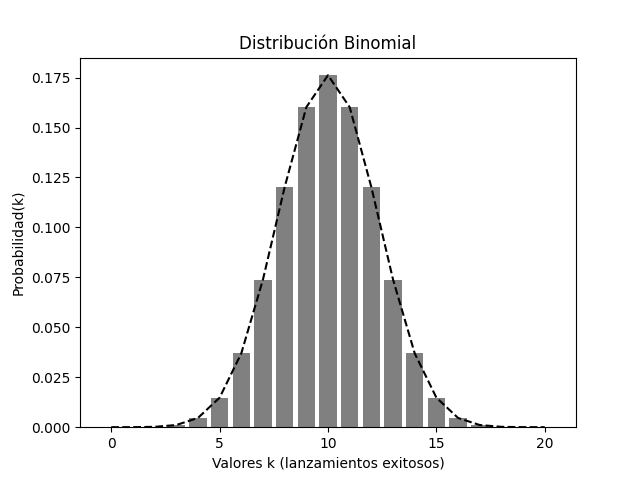
\includegraphics[scale=0.9]{../slides/figures/binomial_distribution_normal.png}
    \label{fig:normal_binomial_distribution}
    \caption{Gráfica de la función de probabilidad binomial con los parámetros $n=20$ y $p=0.5$}
\end{figure}
